\documentclass[a4paper,11pt]{report}
\usepackage[spanish]{babel}
\usepackage[utf8]{inputenc}
\usepackage[margin=1in]{geometry}
\usepackage{lipsum}
\usepackage{hyperref,xcolor,fancyhdr}
\usepackage{graphicx}
\graphicspath{{Figuras/}}
\usepackage{url}
\usepackage{xspace}
\setlength{\parskip}{4mm}
\usepackage{listings}
\definecolor{gray92}{gray}{0.92}
\definecolor{black85}{rgb}{0.28,0.28,0.28}
\hypersetup{
  colorlinks   = true,
  urlcolor     = blue, 
  linkcolor    = black, 
  citecolor   = red 
}

\usepackage{pgfgantt}
\usepackage{pdflscape}




\begin{document}

\begin{titlepage}

\begin{center}
\vspace*{0.5in}
\begin{figure}[htb]
\begin{center}

\includegraphics[width=0.7\textwidth]{uc3m}
\end{center}
\end{figure}
\vspace*{1in}
Universidad Carlos III de Madrid - Escuela Politécnica Superior \\
Grado en Ingeniería Informática \\
Seguridad en dispositivos móviles \\

\vspace*{0.1in}
\emph{Grupo de investigación: Computer Security Lab}  \\

\vspace*{1.2in}
\begin{huge}
\textbf{Android botnets for multi-targeted attacks} \\
\end{huge}


\end{center}

\vfill
\begin{center}
\textbf{Autores:}\\
Adán Cano Moreno - 100346105\\
Jaime García González - 100346062\\
\vspace*{0.2in}
\textbf{Grupo:} 81\\
\vspace*{1in}
\today
\end{center}


\end{titlepage}


\tableofcontents
\thispagestyle{empty}
\chapter{Resumen de tareas}
\renewcommand{\thepage}{\arabic{page}}
\setcounter{page}{1}
\pagestyle{fancy}


%% Descripción de tareas

A continuación, se detallan las tareas realizadas por cada uno de los integrantes del grupo.

\section*{Jaime}

\begin{description}
\item[Trabajos previos.] Lectura de trabajos previos obtenidos de la bibliografía del artículo. Redacción del Capítulo \ref{tPrevios}.
\item[Trabajos posteriores.] Búsqueda y lectura de trabajos posteriores. Redacción del Capítulo \ref{tPosteriores}.
\item[Conclusiones.] Conclusiones obtenidas después de la lectura del artículo principal y de los artículos complementarios. Redacción del Capítulo \ref{conclusiones}.
\item[Planificación.] Realización del diagrama de Gantt de la Sección \ref{planificacion} con la herramienta \emph{pgfgantt}.
\item[Glosario.] Búsqueda de términos importantes del documento y redacción del Apéndice \ref{glosario}.
\item[Bibliografía.] Realización de la bibliografía del documento con la herramienta Bib\LaTeX.
\end{description}

\section*{Adán}

\begin{description}
\item[Introducción.] Tras la lectura del artículo, descripción breve del contenido del mismo de manera objetiva. Redacción del Capítulo \ref{Introduccion}
\item[Revisión crítica del artículo.] Opinión subjetiva del contenido del artículo, indicando tanto sus puntos fuertes como los débiles. Redacción del Capítulo \ref{Critica}
\item[Información básica del autor.] Búsqueda de información respecto al autor del artículo y redacción de la Sección \ref{autor}. 
\item[Información básica de la revista.] Búsqueda de información respecto a la revista donde se publicó el  artículo y redacción de la Sección \ref{revista}. 
\item[Bibliografía.] Realización de la bibliografía del documento con la herramienta Bib\LaTeX.
\end{description}




\chapter{Introducción}\label{Introduccion}

El presente artículo expone el procedimiento a seguir para realizar un ataque \emph{botnet} eficiente sobre diferentes dispositivos móviles \emph{Android} al mismo tiempo para capturar información. El desarrollo del artículo se debe a que cada vez se está realizando un mayor número de ataques con \emph{botnets} a dispositivos móviles, debido a que éstos tienen muchos sensores que son atractivos para los atacantes y a los que se puede acceder de manera sencilla a través de las aplicaciones. 

El principal objetivo del artículo es exponer el potencial que tiene este tipo de ataques y el peligro que puede suponer, puesto que puede ser aplicado para erradicar organizaciones criminales pero también puede ser usado por ciberdelincuentes. En el artículo se muestra un ejemplo de ataque con una \emph{botnet} para mostrar la localización de diferentes dispositivos móviles, describiendo cada fase que hay que realizar. Las fases del ataque son las siguientes:

 
\begin{description}
\item [Recoger información:] Como se puede recoger información de un dispositivo a través de una aplicación \emph{Android}.

\item [Almacenamiento y gestión de la información:] En esta fase se describe el procedimiento a seguir para almacenar la información que ha sido recogida a través del ataque. 

\item [Mostrar la información:] En este fase se describe brevemente como poder mostrar en una página la información que ha sido recogida. 

\item [Información de verificación:] El objetivo de esta fase es conocer el comportamiento de los usuarios que están siendo atacados por una \emph{botnet}. 

\item [Determinar puntos de encuentro entre dispositivos:] En esta fase se describe el proceso para poder determinar el momento en el cual dos dispositivos pueden estar en mismo lugar. 

\end{description}



\chapter{Trabajos previos} \label{tPrevios}

\section{When the Droid became the Bot}

Uno de los grandes problemas de la seguridad en la actualidad ha sido el desarrollo de \emph{botnets}. El \emph{botmaster} despliega el código malicioso a diferentes \emph{hosts} vulnerables. Cuando el sistema ha sido infectado, el dispositivo pasa a formar parte de la \emph{botnet}, comienza a buscar nuevos dispositivos vulnerables y a realizar otras prácticas ilegales.

Las actividades delictivas más habituales que realizan las \emph{botnets} son ataques de \emph{spam} y ataques de denegación de servicio (\emph{DDoS}). En los últimos años, el uso de \emph{smartphones} ha crecido de manera exponencial, por ello, los criminales deciden infectar estos dispositivos para realizar los ataques expuestos anteriormente.

Con la aparición de la tercera generación de redes móviles (3G), los \emph{smartphones} empiezan a conectarse a Internet, con las ventajas y desventajas que implica. Si el dispositivo resulta infectado, el \emph{botmaster} tiene la capacidad de ejecutar diferentes acciones sobre sus esclavos, como pueden ser el envío de SMS, instalar y borrar aplicaciones, realizar llamadas \ldots Aprovechando esta funcionalidad, algunos de los ataques más habituales que ejecutan las \emph{botnets} son los siguientes:

\begin{description}
\item[\emph{Spyware.}] Este tipo de ataques se utiliza para recoger datos personales (nombres, direcciones, datos bancarios \ldots) del atacado. Esto se consigue con la lectura de mensajes, monitorizando la posición del dispositivo, analizando la actividad en Internet y escuchando conversaciones telefónicas.
\item[DDoS.] Ataques de denegación de servicio distribuidos contra \emph{call centers} o diferentes webs.
\item[Ataques al núcleo de la red.] Se realizan ataques de \emph{flooding} a la red celular durante fechas importantes del año, como año nuevo, para colapsar el sistema. Se produce un cuello de botella en el HLR (\emph{Home location register}), que es la base de datos que contiene cada teléfono móvil de la red GSM, hasta forzar su fallo.
\end{description}

En el entorno de pruebas, se han utilizado tres dispositivos \emph{rooteados}, el \emph{botmaster}, la víctima de spam y el dispositivo infectado. El objetivo de la investigación es detectar al \emph{botmaster} analizando los SMS que recibe la víctima.

Se ha analizado el dispositivo afectado, mirando su tarjeta SIM, el almacenamiento interno y su tarjeta SD y no se han encontrado los mensajes de \emph{spam} recibidos. Esto se debe a que el \emph{malware} se ejecuta en las capas intermedias del dispositivo, en vez de en espacio de usuario, véase \ref{botLayer}.

\begin{figure}[htb]
\begin{center}
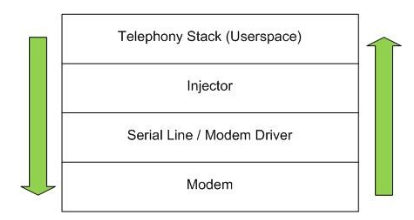
\includegraphics[scale=0.8]{previo1}
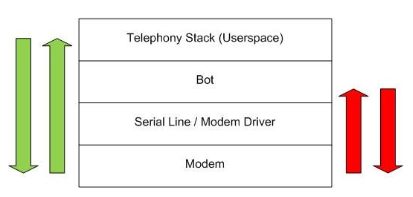
\includegraphics[scale=0.9]{previo2}
\caption{\emph{Bot layer}}
\label{botLayer}
\end{center}
\end{figure}

\section{Andbot: Towards Advanced Mobile Botnets}

Andbot es una \emph{botnet} avanzada que se ejecuta en dispositivos \emph{Android}. Sus características principales son las siguientes:

\begin{description}
\item[Sigilosa.] Utiliza el protocolo HTTP, solo tiene acceso a Internet en segundo plano.
\item[Robusta.] Resistente a la mayoría de técnicas de defensa (sumidero DNS, inyección de comandos, lista negra de IPs \ldots).
\item[Barata.] Bajo coste, bajo uso de datos y bajo gasto energético.
\item[Soporte para comandos.] \emph{Phishing} y filtrado, \emph{DDoS}, robo de información, apagado y control de llamadas.
\end{description}

La parte más importante de una \emph{botnet} es el C\&{}C (\emph{Command and controle design}). Para autenticar comandos, Andbot utiliza el algoritmo RSA. Para enviar comandos a los dispositivos infectados, el \emph{botmaster} genera una imagen JPG en la que se incluye el comando encriptado y firmado, seguidamente se sube a un blog y se comprime la URL. Por otro lado, combina la nueva URL con la fecha de inicio y de expiración del comando. Finalmente, el dispositivo infectado descarga la imagen JPG, descifra el comando y lo ejecuta.

Las pruebas se han realizado en cuatros dispositivos \emph{Android} y se ha incluido el código malicioso dentro de un conocido juego. La primera vez que se ejecuta el juego, Andbot comienza ha realizar sus funciones en segundo plano. Después de reiniciar, el juego se inicia de forma automática y el código se ejecuta siempre que el dispositivo se encuentre en reposo.

Para hacer frente a esta Andbot se recomienda utilizar las técnicas defensivas habituales contra \emph{botnet}, como construir mecanismos de detección coordinados, realizar análisis en busca de comandos que utilicen las vulnerabilidades del sistema y ejecutar por primera vez el código en \emph{sandboxes}.

\section{A K-Means Clustering Algorithm}

El algoritmo K-means \cite{k-means} fue descrito por Hartigan en 1975. Este algoritmo tiene como objetivo dividir un conjunto $MxN$ en $K$ clusters. No se realiza la suma de los cuadrados de todas las particiones, excepto cuando $M$ y $N$ toman valores pequeños y $K=2$. Para el caso general, se busca una solución óptima local que requiera mover un punto de un cluster a otro para evitar la suma de cuadrados \footnote{Si se desea consultar los pasos que realiza el algoritmo, se debe consultar \cite{k-means}.}.

Este algoritmo necesita una serie parámetros de entrada para poder ejecutar correctamente, son los siguientes:

\begin{enumerate}
\item Matriz de entrada de $M$ puntos por $N$ dimensiones.
\item Matriz inicial de $K$ centroides por $N$ dimensiones.
\end{enumerate}


\chapter{Trabajos posteriores} \label{tPosteriores}

En los años siguientes al artículo original, se han realizado multitud de trabajos similares, ya que, el sistema operativo \emph{Android} es cada vez más popular y tiene mayor cuota de mercado. A continuación, se resumen algunos de estos.

\section{Android botnet detection: An integrated source code mining approach}

Este artículo propone diferentes técnicas para detectar las \emph{botnets} en \emph{Android} \cite{posterior1}. Para ello, se aplica ingeniería inversa. Se utiliza la herramienta \emph{dex2jar}, utilizada en el Módulo II, que convierte los ficheros descomprimidos .dex a .jar. Seguidamente, se utiliza la herramienta \emph{JD-GUI} para poder analizar el código fuente del .jar.

Para averiguar si la aplicación contiene código malicioso, se utilizan diferentes modelos predictivos de \emph{machine learning}. Se utilizan técnicas de minería de datos para analizar el código, se realizan estadísticas de las clases analizadas y se buscan palabras clave en el código (\emph{lock}, \emph{concurrent}, etc.). Algunos de los algoritmos que se utilizan en el estudio son:

\begin{itemize}
\item NaiveBayes.
\item K-NN.
\item J48.
\item RandomForest.
\item SMO.
\end{itemize}

Todos los algoritmos tienen un porcentaje de precisión superior al 80 \%{}. Sin embargo, se puede comprobar que el algoritmo que mejor se comporta para detectar código malicioso es el algoritmo K-NN. Los algoritmos se deben entrenar con las nuevas técnicas que implementen las \emph{botnets} para realizar modelos predictivos adecuados.

\section{Investigation into Google Play security mechanisms via experimental botnet}

En este artículo \cite{posterior2}, se introduce código malicioso para que el dispositivo \emph{Android} forme parte de una \emph{botnet} y se comprueban los mecanismos de seguridad que utiliza \emph{Google Play} para publicar aplicaciones.

Se introducen dos componentes en la aplicación, a priori inofensivos, pero que en realidad es el código malicioso de la \emph{botnet}. Se piden los permisos típicos (\emph{GPS}, Internet \ldots) al usuario cuando hace uso de la aplicación, pero, en realidad se utilizan para recopilar información.

El dispositivo infectado recibe un \emph{JSON} del \emph{C\&{}C} en el que se incluyen datos meteorológicos y variables que son utilizadas para configurar y realizar ataques. Se utiliza el algoritmo \emph{SHA-256} para comprobar que las variables de los componentes son iguales que las que recibe del \emph{JSON}.

La aplicación se puede publicar en \emph{Google Play} sin ningún problema, ya que, no se detecta código malicioso. Esto se debe a que la aplicación se conecta con el \emph{C\&{}C} cuando recibe el \emph{JSON}, en la llamada \emph{onCreate()}. Se protegen los componentes maliciosos con cifrado \emph{SHA-256} para evitar que se manipulen.



\chapter{Revisión crítica del artículo}\label{Critica}

La lectura de este artículo nos ha resultado bastante interesante y útil, ya que, trata de un tema tan importante como la seguridad en nuestros dispositivos móviles. Como se ha mencionado en el artículo, cada vez se hace un mayor uso de los \emph{smartphones} y esto hace que los atacantes se sientan atraídos e intenten infectar nuestros dispositivos. Que en un artículo se mencione un procedimiento a través del cual se puede infectar un dispositivo y captar información del mismo hace que el lector se sienta identificado y preste atención al contenido del mismo. Además, pese a que incluye bastante código fuente(lo cuál le hace ser aún más técnico), la mayor parte lectura se nos ha hecho amena y fácil de entender. El artículo está bien estructurado, ya que, después de una breve introducción al mismo, en cada apartado se explica una de las fases del ataque. Esto hace que el lector no pierda en ningún momento la referencia de en que fase del ataque se encuentra. 

Como se ha mencionado antes, la mayor parte de la lectura se ha hecho amena. Sin embargo, a la hora de explicar el proceso de determinar puntos de encuentro a través del algoritmo de k-means la lectura se ha hecho algo más pesada, incluso se ha tenido que volver a leer varias veces más para entender de manera general el desarrollo del algoritmo. 

A pesar de que siempre que pensamos en ataques cibernéticos (en este caso de una \emph{botnet}) pensemos que es para realizar actos delictivos, en el artículo se deja bastante claro que el objetivo de este artículo no es enseñar a realizar un ataque con una \emph{botnet}, si no de analizar el potencial de este sistema para combatir el crimen en el mundo. Por eso, mientras se leía el artículo, no ha dado la sensación de ser un manual para interesados en realizar ataques con una red \emph{botnet}, más bien una manera de describir como nuestro dispositivo puede ser infectado y el peligro que ello conlleva.

Además, a pesar de ser un artículo publicado hace 4 años, este tipo de ataques se siguen dando en la actualidad. Cada vez hay más teléfonos móviles funcionando en el mundo, por lo tanto hay más posibilidades de infectar dispositivos a través de este método y robar información del mismo. Es por ello, por lo que nos ha parecido un artículo interesante, ya que, el hecho de que a pesar del paso del tiempo (unos pocos años en materia de seguridad informática es un mundo) sigue siendo actual y aplicable en estos días.


\chapter{Conclusiones} \label{conclusiones}

 \emph{Android} es un sistema operativo de código abierto que se basa en el \emph{kernel} de Linux, al ser \emph{open soource} tiene una grandísima comunidad detrás que le ofrece soporte, además de ser desarrollado por Google. Por ello, se ha convertido en el sistema operativo móvil más popular y utilizado en el mundo. En el año 2018 tuvo una cuota de mercado superior al 75\%{} en Europa.
 
Por esta razón, muchos hackers implementan código malicioso en aplicaciones para infectar a estos dispositivos. Un ataque muy popular es infectar al dispositivo para que forme parte de una \emph{botnet}, es decir, un conjunto de dispositivos infectados que son controlados por un \emph{botmaster} para realizar ataques a otros dispositivos.

Este tipo de ataques ha estado presente desde la aparición de Internet. Inicialmente, se realizaba en computadoras de sobremesa cuando las redes móviles no ofrecían conexión a Internet. Los objetivos principales de este tipo de ataque son el robo de información personal (\emph{spyware}) y ataques de denegación de servicio distribuidos (\emph{DDoS}) contra servidores de compañías para forzar pérdidas económicas o robo de información.

La aparición del 3G supone un gran avance en telefonía móvil, ya que, permite a los usuarios acceder a Internet desde su dispositivo móvil, con las ventajas y desventajas que supone. La cuarta generación de redes móviles, 4G, mejora los servicios que ofrece el 3G, logrando velocidades de subida y bajada muy superiores.

Los delincuentes utilizan técnicas de ingeniería inversa para decompilar una aplicación confiable, inyectar código malicioso y vuelven a empaquetar para subir la aplicación modificada a la red como si fuese la original. Como se ha podido observar, las técnicas de verificación que utiliza \emph{Google Play} no son perfectas y existen aplicaciones maliciosas en la tienda oficial de aplicaciones. 

Si el dispositivo móvil resulta infectado, el \emph{botmaster} tiene un control total del mismo, teniendo acceso a toda la información personal que contiene. De esta forma, se puede conocer al propietario del dispositivo, conocer sus datos y credenciales bancarias, estudiar su actividad diaria por medio del \emph{GPS} \ldots Por ello, hay que concienciar al usuario para que tenga cuidado cuando descargue aplicaciones poco fiables y le otorgue  permisos, ya que, pone en peligro su privacidad y todos sus datos sensibles.




\bibliography{Bibliografia}
\bibliographystyle{ieeetr}

\appendix

\chapter{Información complementaria}
\section{Información básica del autor}\label{autor}
El autor de este artículo es Valentin Hamon \cite{Autor}. En el momento en el que escribió el artículo era estudiante e investigador del laboratorio de criptologia operacional y virología en ESIEA\cite{ESIEA} (\emph{École supérieure d'informatique, électronique, automatique}. Está graduado como Ingeniero de Seguridad Informática de Sistemas por la ESIEA. Actualmente trabaja en FAMOCO, empresa que ha ha desarrollado la primera solución transaccional Android del mundo para ayudar a las empresas a alcanzar sus objetivos de transformación digital.

Además de este artículo, anteriormente publicó otro titulado: \emph{Malicious URI Resolving in PDFs}, cuyo propósito es mostrar que el simple uso de una petición HTTP desde un PDF puede ser una buena herramienta  para un atacante. Además, este documento trata sobre cómo puede ser relativamente fácil reutilizar algunas vulnerabilidades ajenas al documento. 

\section{Información básica de la revista}\label{revista}

El artículo fue publicado en la revista \emph{Springer-Verlag} \cite{Springer-Verlag}. \emph{Springer-Verlag} es la filial francesa de \emph{Springer}, fundada en 1986. Su sede se encuentra en París. Los temas tratados en sus publicaciones son del ámbito de la medicina, las matemáticas, la estadística, la informática y la ingeniería. Además de la publicación de revistas de carácter científico, \emph{Springer-Verlag} se dedica a la publicación de libros del ámbito de las ciencias y a comercializar la editorial Springer en Francia. 


\section{Planificación} \label{planificacion}

En la siguiente página se muestra la planificación temporal del proyecto realizado, para ello, se ha utilizado un diagrama de Gantt.

\thispagestyle{plain}
\begin{landscape}
  \vspace*{\stretch{1}}
  \resizebox{!}{.76\textheight}{
  \begin{ganttchart}[
  x unit= 28 mm,
  hgrid=true,
  time slot format={little-endian}
  ]{21.03.2019}{31.03.2019} 
  
	\gantttitlecalendar{month=name,day} \\
	
	\ganttmilestone{Inicio del proyecto}{21.03.2019}\\ 
  
	% Lectura y resumen de nuestro artículo
	\ganttgroup{Estudio del artículo}{22.03.2019}{25.03.2019} \\
	\ganttbar[bar/.append style={fill=blue}]{Lectura}{22.03.2019}{23.03.2019}\\
	\ganttbar[bar/.append style={fill=blue}]{Introducción}{23.03.2019}{25.03.2019} \\
	\ganttbar[bar/.append style={fill=blue}]{Datos complementarios}{25.03.2019}{25.03.2019}\\
	
	\ganttgroup{Trabajos previos y posteriores}{24.03.2019}{27.03.2019} \\
	\ganttbar[bar/.append style={fill=red}]{Búsqueda de documentación}{24.03.2019}{25.03.2019}\\
	\ganttbar[bar/.append style={fill=red}]{Lectura}{25.03.2019}{26.03.2019} \\
	\ganttbar[bar/.append style={fill=red}]{Redacción}{26.03.2019}{27.03.2019} \\
	
 
	\ganttgroup{Crítica y conclusión}{28.03.2019}{29.03.2019} \\
	\ganttbar[bar/.append style={fill=orange}]{Revisión crítica}{28.03.2019}{28.03.2019}\\
	\ganttbar[bar/.append style={fill=orange}]{Conclusiones}{29.03.2019}{29.03.2019} \\
	
	\ganttgroup{Preparación del documento}{30.03.2019}{31.03.2019} \\
	\ganttbar[bar/.append style={fill=green}]{Revisión}{30.03.2019}{30.03.2019}\\
	\ganttbar[bar/.append style={fill=green}]{Maquetado}{30.03.2019}{31.03.2019} \\
	
	\ganttmilestone{Entrega del proyecto}{31.03.2019}\\ 
	
	\ganttlink{elem0}{elem1}
	\ganttlink{elem1}{elem5}
	\ganttlink{elem5}{elem9}
	\ganttlink{elem9}{elem12}
	\ganttlink{elem12}{elem15}
  \end{ganttchart}
  }
  \vspace*{\stretch{1}}
\end{landscape}

\chapter{Glosario} \label{glosario}

\begin{description}
\item[Android.] Sistema operativo para dispositivos móviles desarrollado por Google, basado en el kernel de Linux y de código abierto.
\item[API.] Application Programming Interface, conjunto de funciones que ofrece cierta biblioteca para ser utilizado por otro software como capa de abstracción.
\item[Botmaster.]  Individuo o sistema responsable del control de bots.
\item[Botnet.] Conjunto de \emph{bots} que se ejecutan de manera autónoma. El creador de la \emph{botnet} puede controlar los dispositivos infectados de manera remota.
\item[C\&{}C.] Command and Controle, software de control y comandos que utiliza el botmaster para controlar la red.
\item[DDoS.] Distributed Denial of Service, ataque de denegación de servicio que realiza múltiples peticiones hacia un único destino.
\item[DNS.] Domain Name System, sistema de nomenclatura jerárquico descentralizado para dispositivos conectados a redes IP.
\item[GPS.] Global Positioning System, sistema que permite determinar en toda la Tierra la posición de cualquier objeto. 
\item[GSM.] Global System for Mobile, sistema estándar y libre de telefonía digital.
\item[HLR.] Home Location Register, base de datos que contiene todos los dispositivos registrados en la red GSM.
\item[HTTP.] Hypertext Transfer Protocol, protocolo de comunicación que permite la transferencia de datos en la World Wide Web.
\item[IMEI.] International Mobile Equipment Identity, código pregrabado en los móviles GSM que lo identifican unívocamente.
\item[JSON.] JavaScript Object Notation, es un formato de texto sencillo para el intercambio de datos.
\item[Kernel.] Núcleo del sistema operativo.
\item[Machine learning.] Subcampo de las ciencias de la computación y una rama de la inteligencia artificial, cuyo objetivo es desarrollar técnicas que permitan que las computadoras aprendan. 
\item[Phishing.] Proceso de ingeniería social que se utiliza para conseguir datos de usuarios de manera fraudulenta.
\item[Root.] Proceso que permite al usuario tener privilegios elevados (superusuario) para sobrepasar las limitaciones que impone el fabricante de hardware y software en sus dispositivos.
\item[RSA.] Sistema criptográfico de clave pública.
\item[Sandbox.] Aislamiento de procesos, es un mecanismo para ejecutar programas con seguridad y de manera separada.
\item[SHA-256.] Secure Hash Algorithm - 256, función hash de cifrado.
\item[SIM.] Subscriber Identity Module, almacena la clave de servicio del suscriptor usada para identificarse ante la red.
\item[URI.] Uniform Resource Identifier, cadena de caracteres que identifica los recursos de una red de forma unívoca.
\item[URL.]  Uniform Resource Locator, es un identificador de recursos uniforme, URI, cuyos recursos referidos pueden cambiar.
\end{description}


\end{document}


